\section{Course Pages}

\subsection{Course Selection Page}
\subsubsection{Design}
The course selection page provides a home page for students to be able to have an overview of all of their courses. It also provides some other functionality such as showing the most recent announcement, course progress and the most recently accessed topic.
\begin{figure}[h!]
    \centering
    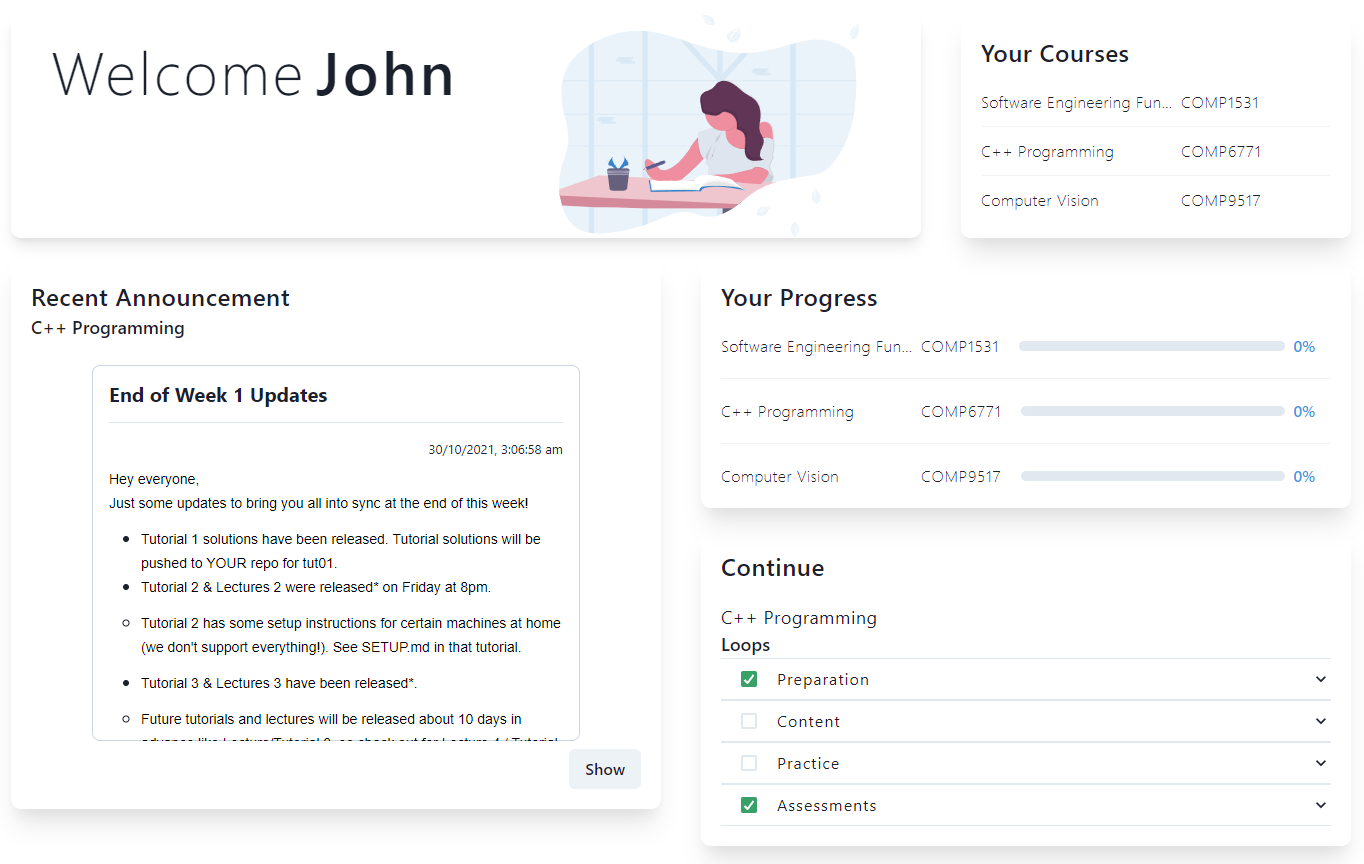
\includegraphics[scale=0.4]{course-selection-page}
    \caption{Student view of the course selection page}
\end{figure}
This is the page that a student will see after signing in.

\subsubsection{Purpose}
The main purpose of this page is to provide users with an overview of their courses. It also is the central page in which users select and traverse into a particular course page.

\subsubsection{What was implemented}
The features within the course selection page that were developed are:
\begin{itemize}
    \item Course selection;
    \item Viewing course progress;
    \item Viewing most recent announcement;
    \item Continuing most recently accessed course content.
\end{itemize}

\subsubsection{How it was implemented}
The course selection page was developed by drafting an overall dashboard UI. The current design utilises a grid based view to separate each feature in boxes.
Each box represents a new feature. The course selection feature was developed by having each course link to the particular course dashboard.
The course progress feature was developed by having the backend database storing each topic and topic content that a user had completed for a particular topic group.
The frontend would then calculate the overall progress of the topic group and then display it on the dashboard.
For the most recent announcement, all announcements from each enrolled course had to be extracted from the backend database. Then the most recent database can be identified and displayed.
The most recently accessed topic is a field that when getting user data would be returned along with the other user information.
This would then allow the dashboard to display the most recently accessed topic for a particular user. When a user clicks on a topic accordion in the course content page this value would change and be updated in the backend database.

\subsubsection{Considerations}
Many considerations had to assessed. The main consideration was identifying what possible features could be added in the dashboard.
The features currently implemented are still in development and can be modified based on what could provide more utility to users.
Other considerations include, what should the dashboard look like for a brand new user or admin?
\begin{figure}[h!]
    \centering
    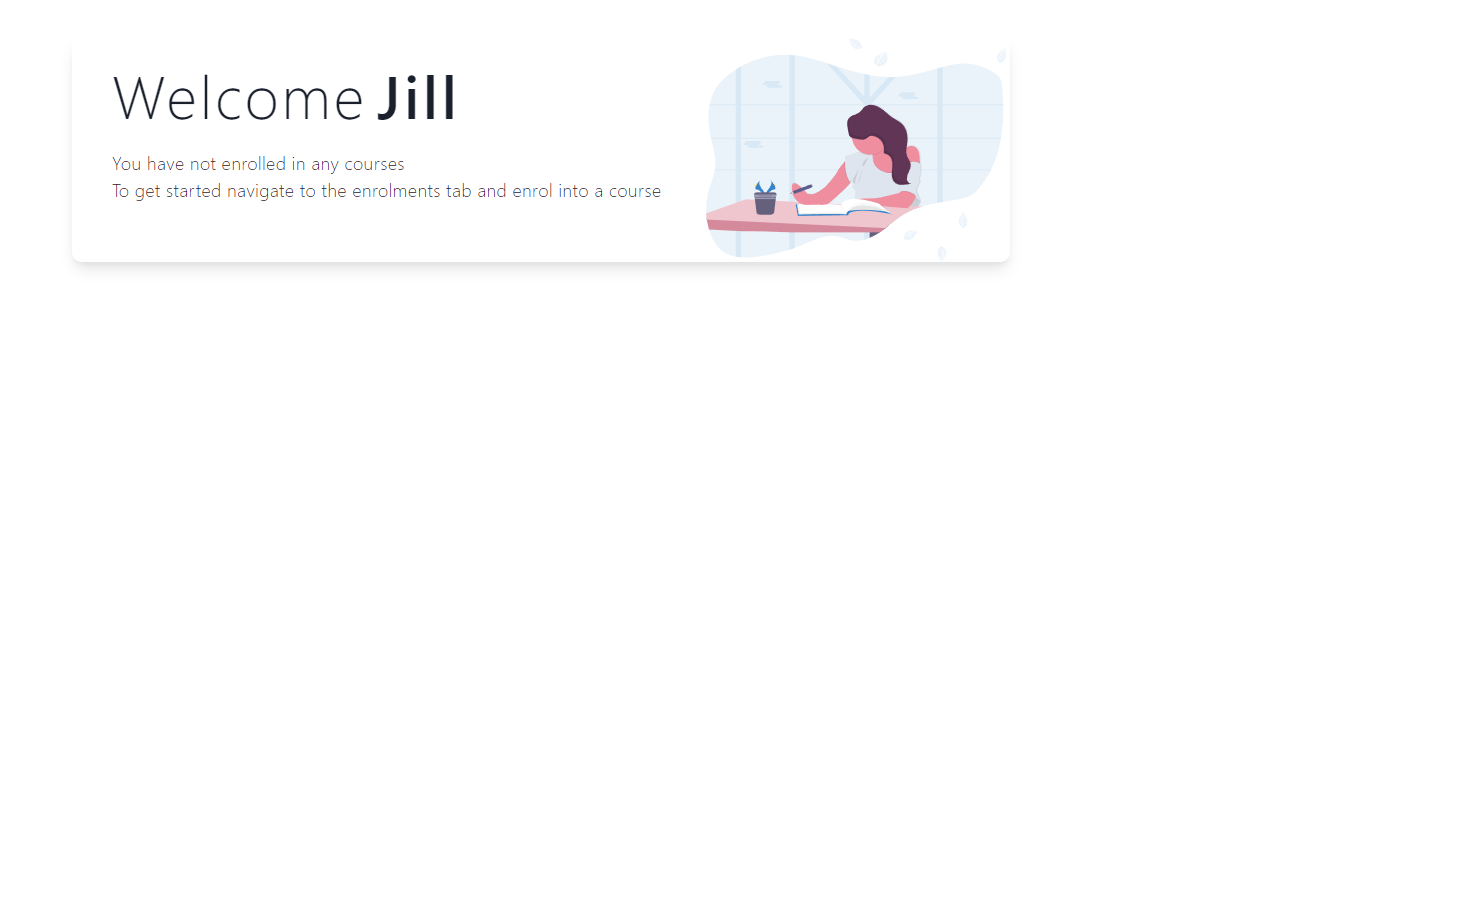
\includegraphics[scale=0.4]{course-dashboard-new-user}
    \caption{New user view of the course selection page}
\end{figure}
\begin{figure}[h!]
    \centering
    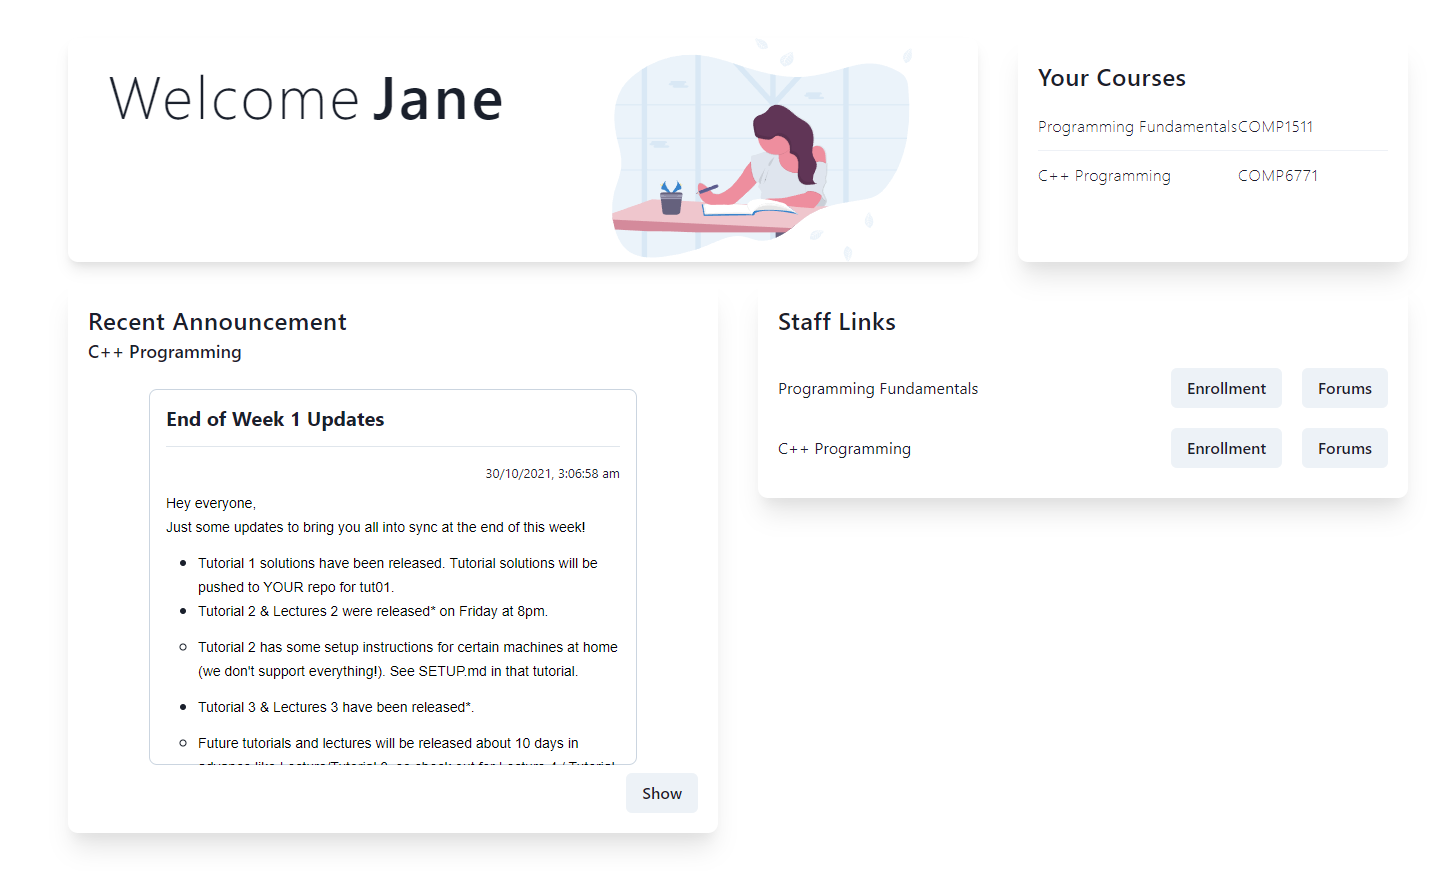
\includegraphics[scale=0.4]{course-selection-admin}
    \caption{Administrator view of the course selection page}
\end{figure}
For a new user, the dashboard will not have any feature, but instead will direct the user to enrol into a course through the enrolment link on the sidebar.
For an administrator, the course progress and most recently accessed topic features will not be displayed, but instead provide the functionality of having links to the forums or enrollment of a particular course.
This feature would benefit an administrator as it would provide a quick and easy way to access those features which an administrator would utilise often.

\subsection{Course Dashboard Page}
\subsubsection{Design}
The course dashboard allows users to view the announcements of the corresponding course and also ask forums questions linked to that particular announcement. For administrators, they can create and update announcemnts.
\begin{figure}[h!]
    \centering
    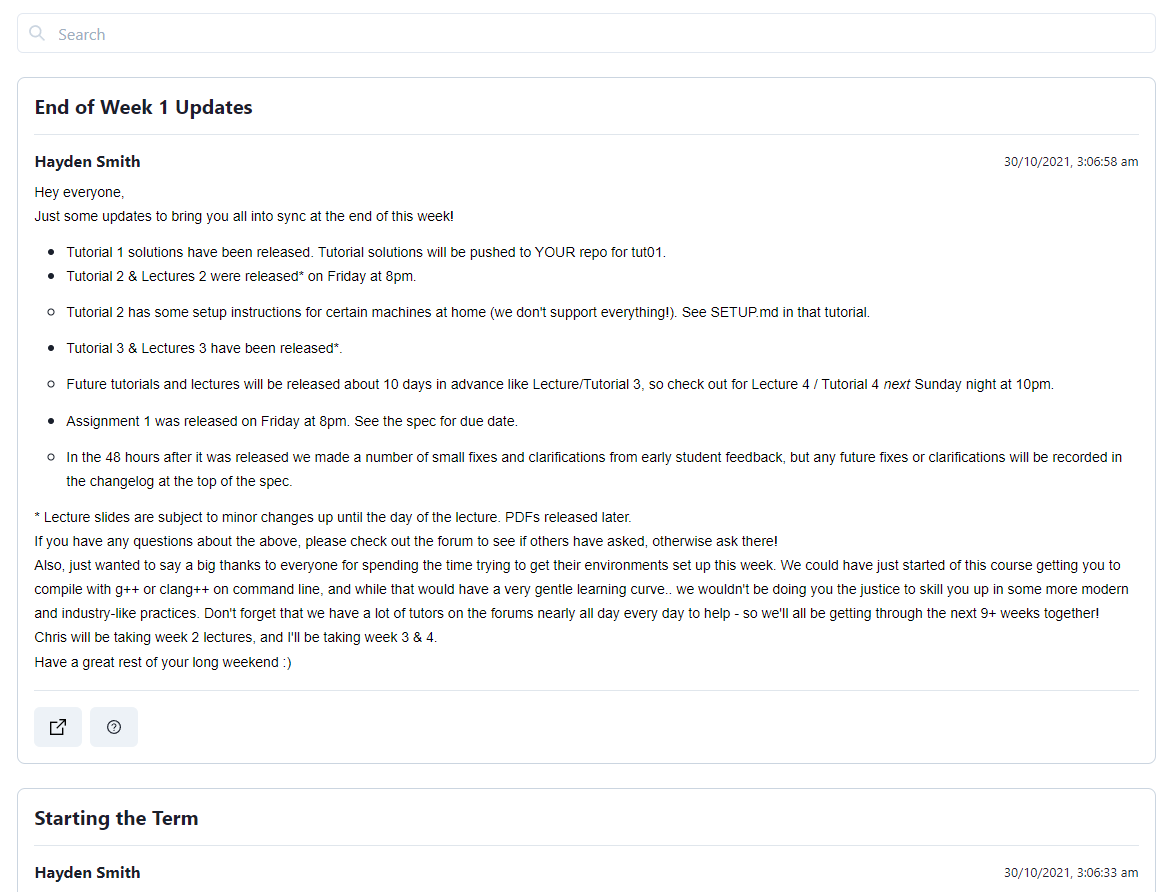
\includegraphics[scale=0.4]{course-dashboard-page}
    \caption{Student view of the course dashboard page}
\end{figure}

\subsubsection{Purpose}
The main purpose of this page was to provide an area for users to view important announcements of a course.
It also allows administrators to create these announcements to notify students.
\subsubsection{What was implemented}
The features that were designed were the ability to view the information of an announcement (title, content, post/edit date and author), the ability to search and filter for announcements and the ability to create and edit announcements as an administrator.
\subsubsection{How it was implemented}
The design of the announcement was implemented in a way to ensure that it would be similiar to a forum post. This would allow users to identify that announcements act similiarly to forums posts.
Thus many of the forum functionality of creating, editting and commenting are very similiar to how the announcement features were developed.
\subsubsection{Considerations}
The main consideration for the course dashboard was determining if a user should be able to directly comment on the course dashboard page or have it be done in the forums page.
The final design has announcement comments linked in the forum so that the forum is the singular area within the course for discussion.
This provides easier use and less confusion for users to swap between pages.

\subsection{Course Content Page}
\subsubsection{Design}
The course content page contains the accordion which displays the topics and corresponding topic content of a particular topic group/course.
\begin{figure}[h!]
    \centering
    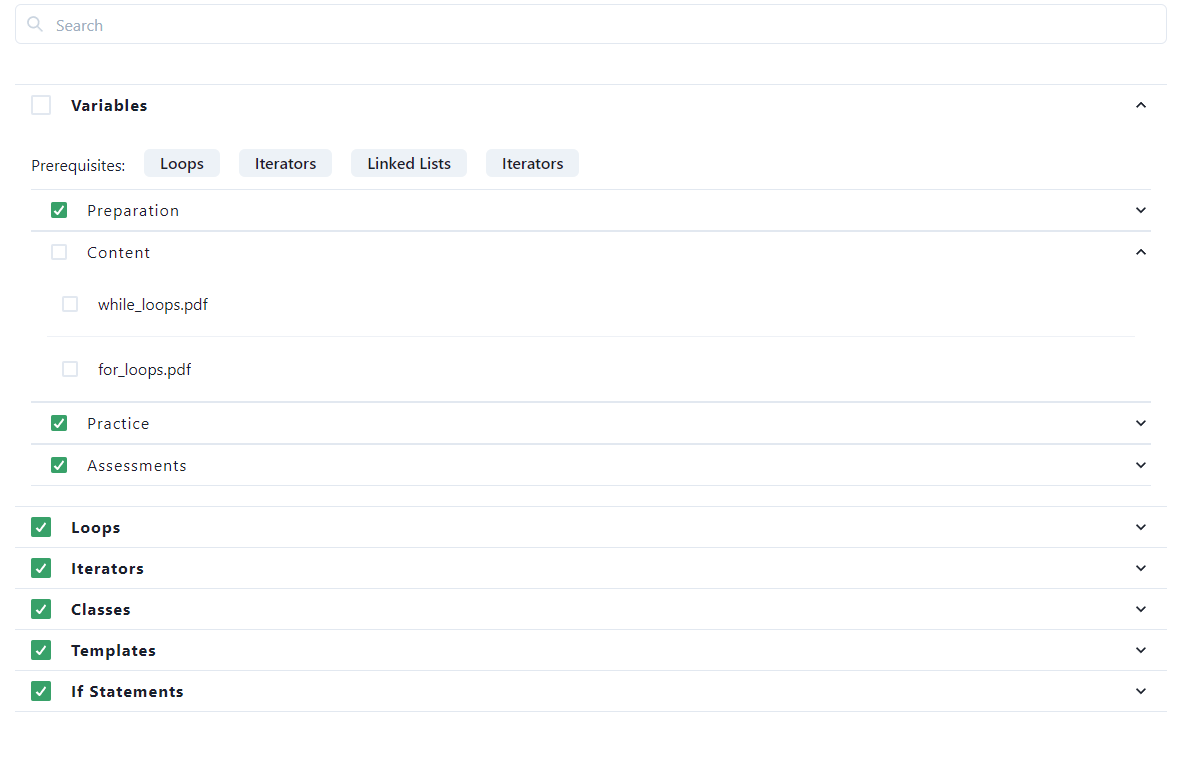
\includegraphics[scale=0.4]{course-content-page}
    \caption{Student view of the course content page}
\end{figure}
\subsubsection{Purpose}
The purpose of the course content page is to provide the topic files of the particular topic group. It is also used to properly categorise the topic files within each topic for a user to learn from.
\subsubsection{What was implemented}
The features that were implemented are displaying the topics and their prerequisites and the ability to search and filter for specific topics.
\subsubsection{How it was implemented}
This page was implemented by first getting all of the topics within the corresponding topic group. Then for each topic categorise each topic file into 4 distinct types, preparation, content, practice and assessments.
The search functionality was implemented by matching any topics or topic files names with the search term.
\subsubsection{Considerations}
A consideration made for the course content page was how to display the topic prerequisites. Since the topic tree displays these topics within a graph with edges to convey prerequisites, a list view needed a way to display the same information.
The current design now uses a list within the topic to display the prerequisites of the corresponding topic.

\subsection{Widgets Bar}
\subsubsection{Design}
The widgets bar exists on the right hand side of both the main selection page and the course pages.
\begin{figure}[h!]
    \centering
    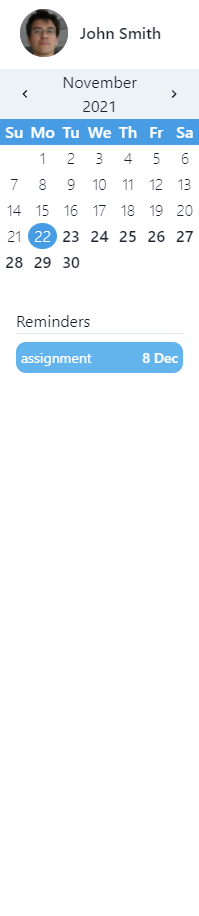
\includegraphics[scale=0.4]{widgets-bar}
    \caption{Widgets bar}
\end{figure}
\subsubsection{Purpose}
The purpose of the widgets bar is to provide extra utility for users. 
\subsubsection{What was implemented}
The features of the widgets bar include the calendar feature, account section and the reminders list. The calendar feature allows users to create reminders on the calendar UI, these reminders will then be displayed on the reminder. The account section provides an area for users to log out and view their account.
\subsubsection{How it was implemented}
Since most pages within the metaLMS contain the sidebars, a universal template page was created with both side bars present and the main content of the page changing based on the route URL.
The widgets bar utilise a calendar which allows users to click on a particular date and create a reminder which is stored in the database. These reminders would then be shown on the reminders list, with a maximum of 5 showing at a time.
Users can also delete reminders.
\subsubsection{Considerations}
The main consideration for the widgets bar was to determine what features to add to the side bar. Due to the limited space, careful consideration was made, however possible additions can still be added.